\chapter{Kết luận và Hướng phát triển}
\label{chap:conclusion}

\section{Tổng kết kết quả đạt được so với mục tiêu đề ra}

Đồ án tốt nghiệp này đã thiết kế, hiện thực hóa và đánh giá thực nghiệm \textbf{CITRA} (\textit{Essay Integrity Checker v3.90.3}) --- một nền tảng phần mềm kết hợp nơ-ron -- ký hiệu (neuro-symbolic) có khả năng giải thích, phục vụ chấm điểm tự động tính toàn vẹn trích dẫn (Citation Integrity Scoring -- CIS), phát hiện tài liệu tham khảo ngụy tạo và chuẩn hóa danh mục tài liệu tham khảo. Bảng~\ref{tab:obj-summary} đối chiếu trực tiếp các sản phẩm phần mềm đã hoàn thiện cùng kết quả thực nghiệm đạt được với sáu mục tiêu nghiên cứu đề ra tại Mục~\ref{sec:objectives}.

{\setlength{\tabcolsep}{3.5pt}
\begin{longtable}{|C{0.14}|L{0.32}|L{0.54}|}
\caption{Tổng hợp kết quả đạt được của đồ án tốt nghiệp đối chiếu với các mục tiêu tại Chương 1.}\label{tab:obj-summary}\\
\hline
\textbf{Mục tiêu} & \textbf{Năng lực mục tiêu} & \textbf{Kết quả kỹ thuật và thực nghiệm đạt được} \\
\hline
\endfirsthead
\multicolumn{3}{l}{\itshape Bảng \thetable\ (tiếp theo trang trước)}\\
\hline
\textbf{Mục tiêu} & \textbf{Năng lực mục tiêu} & \textbf{Kết quả kỹ thuật và thực nghiệm đạt được} \\
\hline
\endhead
\hline
\multicolumn{3}{r}{\itshape Tiếp theo ở trang sau}\\
\endfoot
\hline
\endlastfoot
\textbf{OBJ-1} & Trích xuất đa định dạng và liên kết hai chiều & Kết hợp lai GROBID \texttt{0.9.1-crf} TEI-XML + PyMuPDF + \texttt{python-docx} hỗ trợ 12 chuẩn trích dẫn (gồm cả văn bản pháp luật VN) và bộ liên kết 7 phương pháp (phát hiện mục tài liệu tham khảo đạt $97.7\%$--$100\%$ trên 310 tệp PDF). \\
\hline
\textbf{OBJ-2} & Truy xuất liên hợp nhận biết miền tri thức & Kho dữ liệu cục bộ SQLite FTS5 gồm 129,125 bản ghi (độ phủ $99.80\%$, độ trễ $87.6\text{\,ms}$) kết hợp hơn 15 API trực tuyến, Retraction Watch, bộ nhớ đệm gộp truy vấn singleflight và bộ kiểm tra URL/HTML ghim địa chỉ IP. \\
\hline
\textbf{OBJ-3} & Xác minh nơ-ron -- ký hiệu và hiệu chỉnh xác suất & Bộ mã hóa kép SBERT + ONNX INT8 \texttt{VI}$\leftrightarrow$\texttt{EN} tích hợp cùng 68 luật ký hiệu, mô hình hồi quy logistic đa thức 16 chiều ($C=2.0$) và hiệu chỉnh Platt ($\text{ECE} = 0.0395$, $\text{Brier} = 0.0125$). \\
\hline
\textbf{OBJ-4} & Chấm điểm CIS minh bạch và sửa lỗi tự động & Thang chấm CIS năm thành phần (độ ổn định thứ hạng $\rho = 0.9987$) đi kèm tính năng tự động chuẩn hóa và sửa lỗi tài liệu tham khảo theo chuẩn APA, IEEE, TDTU, BibTeX, RIS và tệp \texttt{.docx}. \\
\hline
\textbf{OBJ-5} & Nền tảng web phân quyền bảo mật & Hệ thống FastAPI đóng gói bằng container (15 bảng ORM, 13 bản di trú lược đồ (\texttt{0001}--\texttt{0013}), SSE, bảo vệ RBAC/IDOR, chống SSRF bằng ghim IP) và ứng dụng đơn trang React 18.3 (gói khởi tạo $228.42\text{\,kB}$). \\
\hline
\textbf{OBJ-6} & Đánh giá thực nghiệm quy mô lớn chống rò rỉ dữ liệu & Độ chính xác trong phân phối (ID) đạt $99.02\%$ ($N=18\text{K}$), ngoài phân phối (OOD) đạt $99.75\%$ ($N=2.4\text{K}$), đánh giá đầu-cuối (E2E) trên 6 lĩnh vực đạt $100\%$ ($120/120$) và chịu tải đồng thời $50/50$ phiên. \\
\hline
\end{longtable}
}

Hình~\ref{fig:verdict-paths} tổng hợp cơ chế bảo vệ kiến trúc cốt lõi chi phối mọi phán quyết trong \textbf{CITRA}: các kết luận nghi ngờ ngụy tạo (\texttt{suspected\_hallucination}) bắt buộc phải dựa trên bằng chứng bác bỏ cấu trúc xác thực (mã DOI ngụy tạo hoặc chắp vá chéo, tên miền giả lập theo RFC 2606, năm xuất bản phi lý ở tương lai) hoặc phản hồi rỗng hợp lệ với mã trạng thái HTTP 200 đồng nhất từ nhiều cơ sở dữ liệu học thuật trực tuyến; ngược lại, các trường hợp cạn kiệt hạn ngạch mạng, mã DOI khu vực chưa công bố siêu dữ liệu hay độ tương đồng nằm trong vùng biên ($[0.40, 0.60)$) đều được điều hướng tất định về trạng thái \texttt{unresolved} để giảng viên trực tiếp xem xét.

\begin{figure}[H]
    \centering
    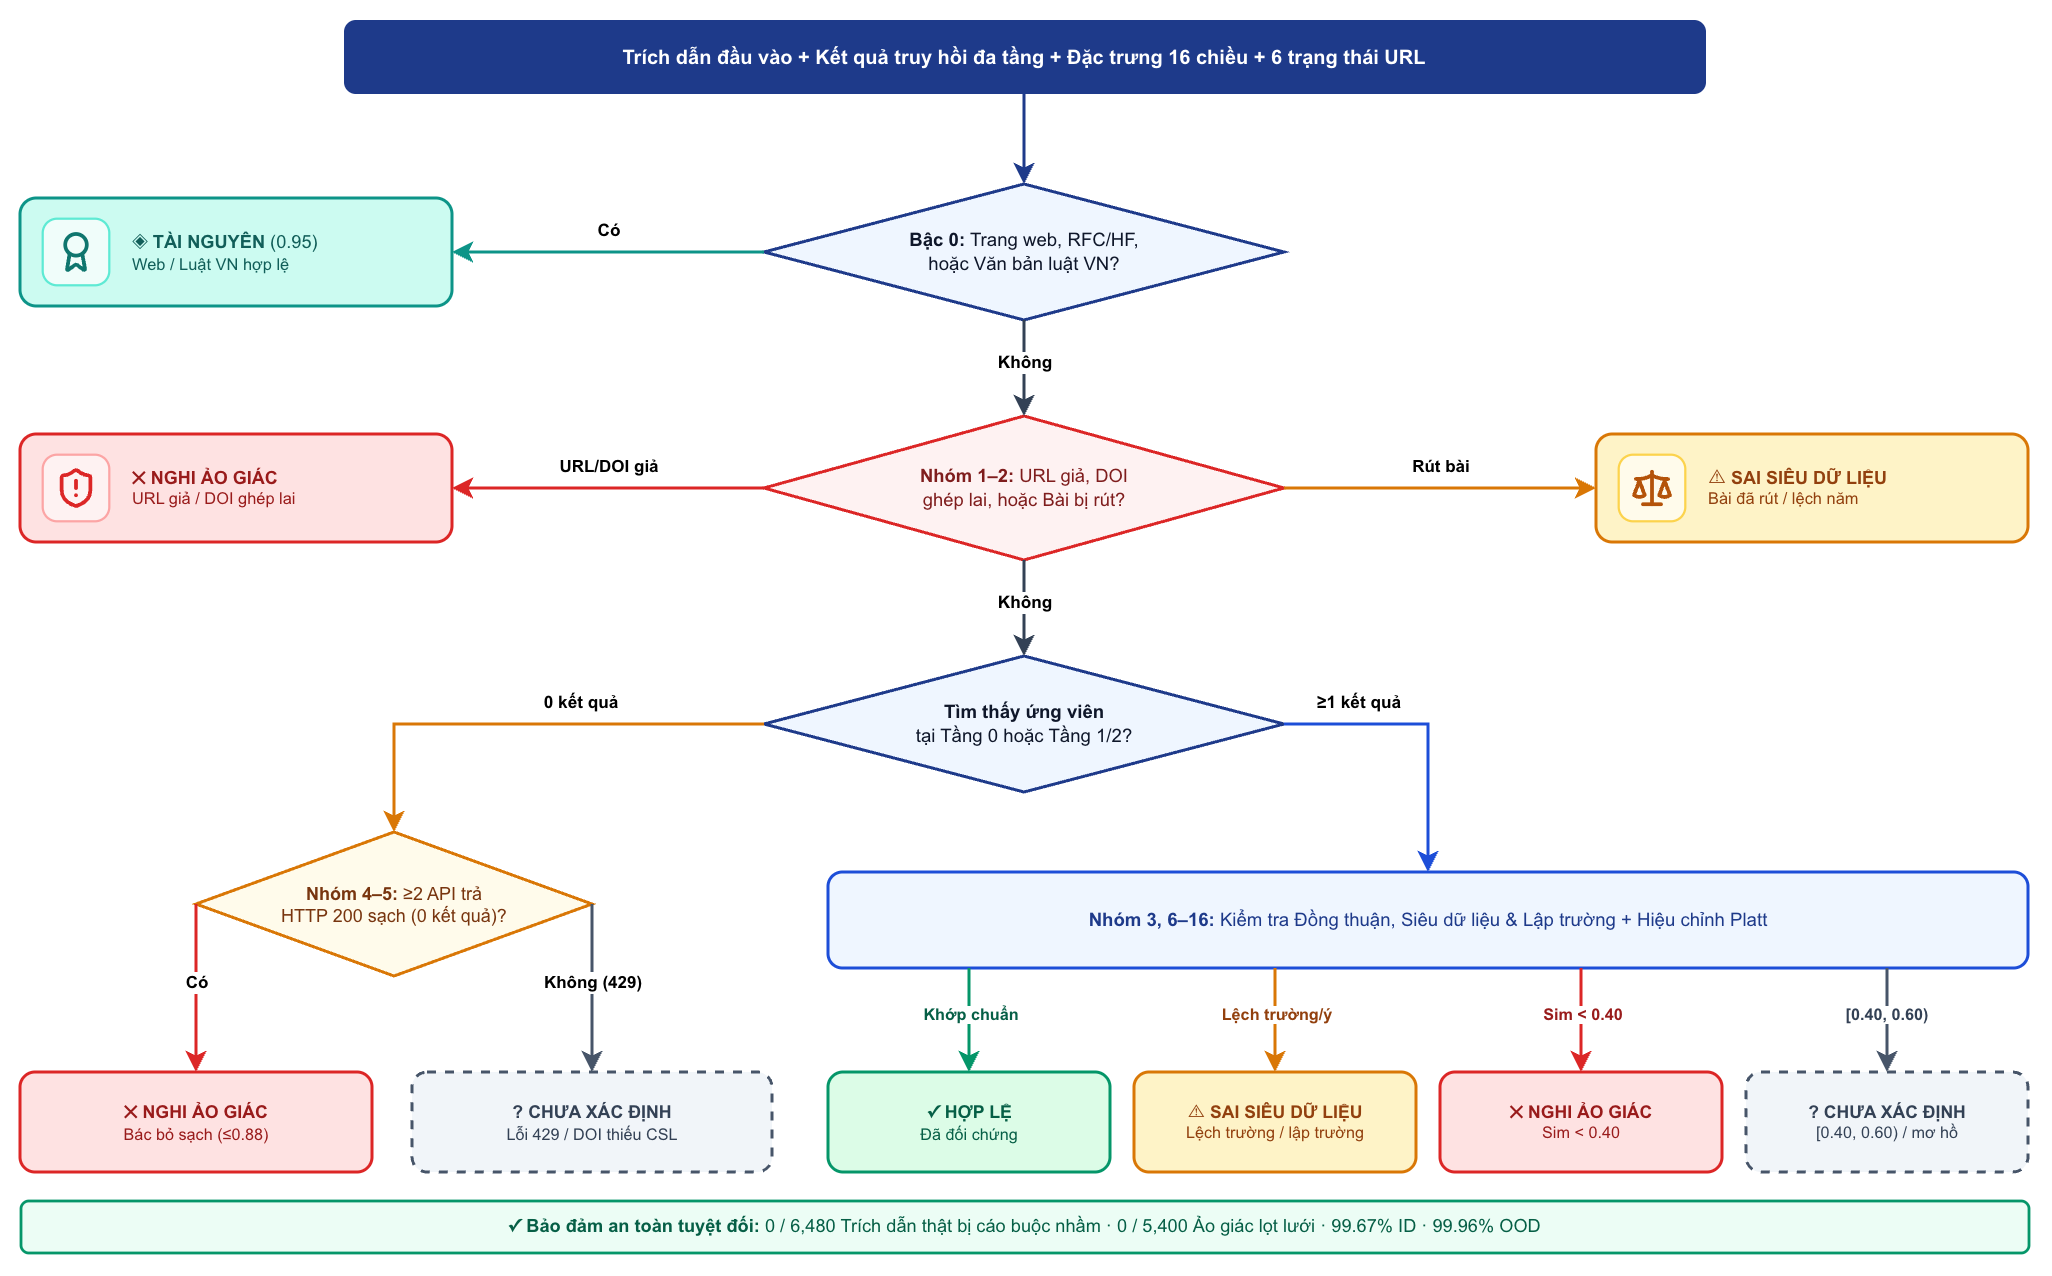
\includegraphics[width=\textwidth,keepaspectratio]{picture/figures/fig6_1_verdict_paths.png}
    \caption[Cây quyết định nơ-ron -- ký hiệu có rào chắn phân tách bác bỏ và từ chối phán quyết]{Cây quyết định nơ-ron -- ký hiệu có rào chắn bảo vệ trong CITRA (\texttt{v3.90.3}) giúp phân tách rạch ròi giữa kết luận bác bỏ có bằng chứng (\texttt{suspected\_hallucination}) và cơ chế từ chối phán quyết có truy vết nguồn gốc (\texttt{unresolved}).}
    \label{fig:verdict-paths}
\end{figure}

\section{Tổng hợp các phát hiện thực nghiệm trọng tâm}

Ba bài học thực nghiệm quan trọng được rút ra từ chuỗi thí nghiệm tại Chương~\ref{chap:results}:
\begin{enumerate}
    \item \textbf{Hệ luật ký hiệu và học thống kê bổ trợ lẫn nhau thay vì dư thừa.} Mô hình Hồi quy Logistic 16 chiều thuần túy (\texttt{B5}) hoạt động tốt trên các biên đánh đổi độ tương đồng liên tục ($97.98\%$ trên tập ID) nhưng sụt giảm nghiêm trọng xuống chỉ còn $49.88\%$ trước các quy tắc toàn vẹn rời rạc ngoài phân phối OOD (như bài báo đã bị rút bỏ hoặc mã DOI chắp vá chéo). Việc kết hợp các rào chắn luật ký hiệu có thứ tự ưu tiên cùng cơ chế pha trộn xác suất học máy giúp hệ thống đạt đồng thời $99.02\%$ độ chính xác ID và $99.75\%$ độ chính xác OOD.
    \item \textbf{Hiệu chỉnh xác suất hậu kiểm là yếu tố thiết yếu để báo cáo độ tin cậy đáng tin.} Điểm tự tin thô sinh ra trực tiếp từ tập luật ký hiệu mắc hiện tượng tự tin thái quá nghiêm trọng ($\text{ECE} = 0.2445$). Phép hiệu chỉnh Platt trên không gian logit giúp giảm sai số hiệu chỉnh kỳ vọng (ECE) tới $6.19\times$, xuống còn $0.0395$, trong khi vẫn bảo toàn nguyên vẹn tỷ lệ bao phủ không từ chối phán quyết ($87.91\%$).
    \item \textbf{Chỉ mục FTS5 ngoại tuyến giúp việc triển khai thực tế tại lớp học trên máy chủ thuần CPU trở nên khả thi.} Cơ chế lưu đệm ứng viên đã xác minh kết hợp lập chỉ mục cục bộ 129,125 bài báo mang lại tốc độ truy xuất nhanh hơn $688.72\times$, cho phép một máy chủ chỉ sử dụng CPU xử lý trọn vẹn 50 lượt tải bài đồng thời vào thời điểm sát hạn nộp mà không gặp tình trạng sụp đổ do giới hạn tần suất từ các API bên ngoài.
\end{enumerate}

\section{Hạn chế của hệ thống}
\label{sec:limitations}

Mặc dù đạt hiệu năng thực nghiệm ấn tượng, phiên bản \texttt{3.90.3} hiện vẫn tồn tại bốn hạn chế kỹ thuật cụ thể:
\begin{itemize}
    \item \textbf{L1 (Điểm mù đối chứng luận điểm trên toàn văn có thu phí):} Cơ chế đối sánh ngữ nghĩa hiện tại so khớp câu trích dẫn trong bài với tiêu đề và phần tóm tắt mở (abstract). Khi sinh viên trích dẫn một hình vẽ, định lý hoặc đoạn thảo luận chi tiết nằm sâu bên trong bài báo đóng phí truy cập mà phần tóm tắt không đề cập tới, \textbf{CITRA} chưa thể kiểm chứng quan hệ suy diễn ngữ nghĩa ở cấp độ toàn văn.
    \item \textbf{L2 (Độ lệch lĩnh vực trong kho dữ liệu ngoại tuyến):} Do $98.43\%$ dữ liệu trong \texttt{local\_papers.db} bắt nguồn từ ACL Anthology và kho bài báo Khoa học Máy tính trên arXiv, các môi trường triển khai cô lập hoàn toàn không có kết nối Internet sẽ bị giảm độ phủ truy xuất Tầng 0 (Tier-0) đối với các bài báo thuộc lĩnh vực y sinh, khoa học xã hội -- nhân văn và các tạp chí chuyên ngành xuất bản trong nước tại Việt Nam.
    \item \textbf{L3 (Tài liệu lưu trữ đa cột phức tạp và bản quét chữ viết tay):} Dù cơ chế nhận dạng ký tự quang học (Tesseract OCR) có chọn lọc đã khôi phục tốt các trang in tiếng Việt, những bản chụp bằng camera độ phân giải thấp, tài liệu lưu trữ bị nghiêng lệch hoặc ghi chú trích dẫn viết tay bên lề vẫn làm suy giảm độ chính xác nhận dạng ký tự và làm tăng tỷ lệ phân loại vào nhóm \texttt{unresolved}.
    \item \textbf{L4 (Tuần tự hóa tác vụ ghi của SQLite trên một máy chủ đơn lẻ):} Mặc dù chế độ SQLite WAL đáp ứng tốt 50 lượt sinh viên tải bài đồng thời trên một máy chủ duy nhất, việc mở rộng theo chiều ngang (horizontal scaling) qua nhiều máy ảo API độc lập đòi hỏi một hệ quản trị cơ sở dữ liệu quan hệ dùng chung qua mạng cùng hệ thống hàng đợi thông điệp phân tán.
\end{itemize}

\section{Hướng phát triển}
\label{sec:future-work}

Mỗi hạn chế nêu tại Mục~\ref{sec:limitations} trực tiếp mở ra một định hướng phát triển kỹ thuật tương ứng trong tương lai:
\begin{itemize}
    \item \textbf{F1 (Truy xuất đoạn văn toàn văn truy cập mở $\leftarrow$ L1):} Tích hợp dữ liệu JATS XML từ PubMed Central, HTML5 từ arXiv (\texttt{ar5iv}) và tệp PDF truy cập mở từ Unpaywall kết hợp truy xuất đoạn văn dày đặc (dense passage retrieval) ở cấp độ đoạn văn, giúp mở rộng khả năng kiểm chứng luận điểm vượt ra ngoài phạm vi tóm tắt bất cứ khi nào giấy phép mở cho phép.
    \item \textbf{F2 (Mở rộng kho dữ liệu ngoại tuyến đa ngành và khu vực ASEAN $\leftarrow$ L2):} Bổ sung vào \texttt{local\_papers.db} các bản chụp dữ liệu mở từ DOAJ, Cơ sở dữ liệu Tạp chí Khoa học Việt Nam Trực tuyến (VJOL) và các phân vùng chuyên ngành của OpenAlex nhằm cân bằng độ phủ ngoại tuyến trên các lĩnh vực kinh tế, luật học, y sinh và kỹ thuật.
    \item \textbf{F3 (Nhận dạng OCR thị giác -- ngôn ngữ nhận biết bố cục $\leftarrow$ L3):} Tích hợp các mô hình phân tích bố cục tài liệu gọn nhẹ đã lượng tử hóa cho CPU (như Docling hoặc Surya OCR) nhằm nâng cao chất lượng phân tách tài liệu tham khảo trên các bản quét lưu trữ kém chất lượng và các bản thảo nhân văn sử dụng nhiều chú thích cuối trang phức tạp.
    \item \textbf{F4 (Mở rộng cụm tiến trình PostgreSQL + Redis và tích hợp LMS chuẩn LTI 1.3 $\leftarrow$ L4):} Hỗ trợ tùy chọn vùng kết nối PostgreSQL (connection pooling) và hàng đợi tác vụ Redis song song với giao thức Learning Tools Interoperability (LTI 1.3) đồng bộ trực tiếp vào sổ điểm của Moodle và Canvas, tạo tiền đề triển khai các nghiên cứu theo dõi dài hạn liên khoa qua nhiều học kỳ.
\end{itemize}

\section{Lời kết}

Các công cụ phần mềm phục vụ đánh giá học thuật luôn mang trên mình trách nhiệm về tính công bằng và sự minh bạch. Bằng cách đặt mọi phép kiểm tra trích dẫn trên nền tảng các cơ sở dữ liệu học thuật có thể truy vết rõ ràng, kết hợp đối sánh ngữ nghĩa bằng mạng nơ-ron với 68 luật ký hiệu có thể kiểm toán cùng xác suất đã hiệu chỉnh Platt, trung thực từ chối đưa ra phán quyết khi bằng chứng chưa đầy đủ và trao quyền quyết định ghi đè cuối cùng cho giảng viên, \textbf{CITRA} đã minh chứng một bản thiết kế kỹ thuật phần mềm thiết thực cho bài toán xác minh liêm chính học thuật có sự hỗ trợ đáng tin cậy của trí tuệ nhân tạo.
